\documentclass[11pt,a4paper]{article}
\usepackage[margin=2.5cm,headheight=15pt]{geometry}
\usepackage{amsmath,amssymb,amsthm}
\usepackage{mathtools}
\usepackage{microtype}
\usepackage{hyperref}
\usepackage{cleveref}
\usepackage{enumitem}
\usepackage{mdframed}
\usepackage{xcolor}
\usepackage{titlesec}
\usepackage{booktabs}
\usepackage{tikz}
\usetikzlibrary{positioning,arrows.meta,shapes.geometric,calc}
\usepackage{fancyhdr}

\definecolor{navyblue}{RGB}{26,58,92}
\definecolor{midblue}{RGB}{44,95,138}
\definecolor{lightblue}{RGB}{232,240,248}
\definecolor{proofgray}{RGB}{242,242,242}

\hypersetup{colorlinks=true,linkcolor=midblue,citecolor=midblue,urlcolor=midblue}

\pagestyle{fancy}\fancyhf{}
\fancyhead[L]{\small\color{navyblue}\textit{SSP–GTSP Structural Equivalences}}
\fancyhead[R]{\small\color{navyblue}\thepage}
\renewcommand{\headrulewidth}{0.4pt}

\titleformat{\section}{\large\bfseries\color{navyblue}}{}{0em}{}[\color{navyblue}\titlerule]
\titleformat{\subsection}{\normalsize\bfseries\color{midblue}}{}{0em}{}

\newmdenv[backgroundcolor=lightblue,linecolor=navyblue,linewidth=1.2pt,
  leftline=true,rightline=false,topline=false,bottomline=false,
  innerleftmargin=12pt,innerrightmargin=8pt,innertopmargin=8pt,
  innerbottommargin=8pt,skipabove=10pt,skipbelow=6pt]{thmbox}

\newmdenv[backgroundcolor=proofgray,linecolor=midblue,linewidth=0.8pt,
  leftline=true,rightline=false,topline=false,bottomline=false,
  innerleftmargin=10pt,innerrightmargin=8pt,innertopmargin=6pt,
  innerbottommargin=6pt,skipabove=6pt,skipbelow=6pt]{proofbox}

\theoremstyle{plain}
\newtheorem{theorem}{Theorem}[section]
\newtheorem{lemma}[theorem]{Lemma}
\newtheorem{corollary}[theorem]{Corollary}
\theoremstyle{definition}
\newtheorem{definition}[theorem]{Definition}
\newtheorem{remark}[theorem]{Remark}

\setlist[itemize]{noitemsep,topsep=4pt}
\setlist[enumerate]{noitemsep,topsep=4pt}

% ─────────────────────────────────────────────────────────────────────────────
\begin{document}
% ─────────────────────────────────────────────────────────────────────────────

\begin{center}
  {\color{navyblue}\rule{\textwidth}{2pt}}\\[0.4cm]
  {\LARGE\bfseries\color{navyblue}The Job Sequencing and Tool Switching Problem}\\[0.3cm]
  {\large\itshape\color{midblue}Part III: SSP–GTSP Structural Equivalences}\\[0.2cm]
  {\color{navyblue}\rule{\textwidth}{2pt}}
\end{center}

\begin{mdframed}[backgroundcolor=lightblue,linecolor=navyblue,linewidth=1pt,
  innerleftmargin=14pt,innerrightmargin=14pt,innertopmargin=8pt,innerbottommargin=8pt]
\small\textbf{Scope.}
This document establishes the formal structural relationship between the U-SSP
and the Generalized Traveling Salesman Problem (GTSP).
We prove: (1) a forward polynomial reduction from SSP to GTSP via the
Intersecting-to-Nonintersecting (I-N) transformation;
(2) a \emph{Disjointness Condition} identifying when SSP is natively a GTSP;
(3) a \emph{Metric Barrier} showing that the reverse reduction does not hold
in general.
These results justify using GTSP solvers (Concorde, LKH) on the configuration graph.
\end{mdframed}

\vspace{0.5cm}
\tableofcontents
\newpage

% ─────────────────────────────────────────────────────────────────────────────
\section{The GTSP and the Overlap Problem}
\label{sec:gtsp_overlap}
% ─────────────────────────────────────────────────────────────────────────────

\begin{definition}[Generalized TSP (GTSP)]
Given a complete graph on vertex set $V$ partitioned into disjoint clusters
$V_1,\ldots,V_n$ with edge costs $w:V\times V\to\mathbb{R}_{\ge 0}$, find a
minimum-cost Hamiltonian cycle that visits \emph{exactly one vertex from each cluster}.
\end{definition}

The non-compact SSP formulation in \texttt{02\_noncompact\_formulation.tex} looks
like a GTSP: the configuration space $\mathcal{C}$ is the vertex set, job clusters
$H_j$ play the role of the GTSP clusters, and $d(C_u,C_v)=b-|C_u\cap C_v|$ gives
edge costs. The objective is to find a minimum-cost path (cycle through a depot)
that visits at least one configuration per job cluster.

However, a direct mapping to a standard GTSP solver is blocked by the
\textbf{Overlap Problem}: in the SSP, a single configuration $C$ may belong to
multiple clusters simultaneously (if $T_i \cup T_j \subseteq C$ for distinct jobs
$i,j$), whereas the GTSP requires \emph{disjoint} clusters. Standard GTSP solvers
assume that selecting a vertex satisfies exactly one cluster; applying them
naively to overlapping clusters produces incorrect results.

% ─────────────────────────────────────────────────────────────────────────────
\section{The I-N Transformation: SSP $\to$ GTSP}
\label{sec:in_transform}
% ─────────────────────────────────────────────────────────────────────────────

The Intersecting-to-Nonintersecting (I-N) transformation \cite{Lien1993} resolves
the Overlap Problem by replicating each configuration once per job it can serve.

\subsection{Construction}

Given a U-SSP instance $\mathcal{I}_{\text{SSP}} = \langle J, T, b, \{T_j\} \rangle$,
construct the GTSP instance $\mathcal{I}_{\text{GTSP}} = \langle V^*, \mathcal{E}^*, d^*, \{V_j^*\} \rangle$ as follows.

\begin{enumerate}
\item \textbf{Vertex replication.}
For each job $j \in J$, create a disjoint cluster:
\[
  V_j^* = \{ v_{C,j} \mid C \in H_j \} \quad \forall j \in J.
\]
Each configuration $C$ that can process multiple jobs spawns multiple distinct
replicas (one per job). This guarantees $V_i^* \cap V_j^* = \emptyset$ for $i \ne j$.

\item \textbf{Inter-cluster arc costs.}
For two replicas in different clusters, inherit the original metric:
\[
  d^*(v_{C_u,i},\, v_{C_w,j}) = d(C_u, C_w) = b - |C_u \cap C_w|
  \quad \forall i \ne j.
\]

\item \textbf{Zero-cost intra-configuration arcs.}
If the same configuration $C$ is replicated in two different clusters $V_i^*$
and $V_j^*$, connecting the two replicas has zero cost:
\[
  d^*(v_{C,i},\, v_{C,j}) = b - |C \cap C| = b - b = 0.
\]
These zero-cost arcs model the fact that processing multiple consecutive jobs
under the \emph{same} magazine configuration incurs no tool switch.
\end{enumerate}

\begin{figure}[h!]
\centering
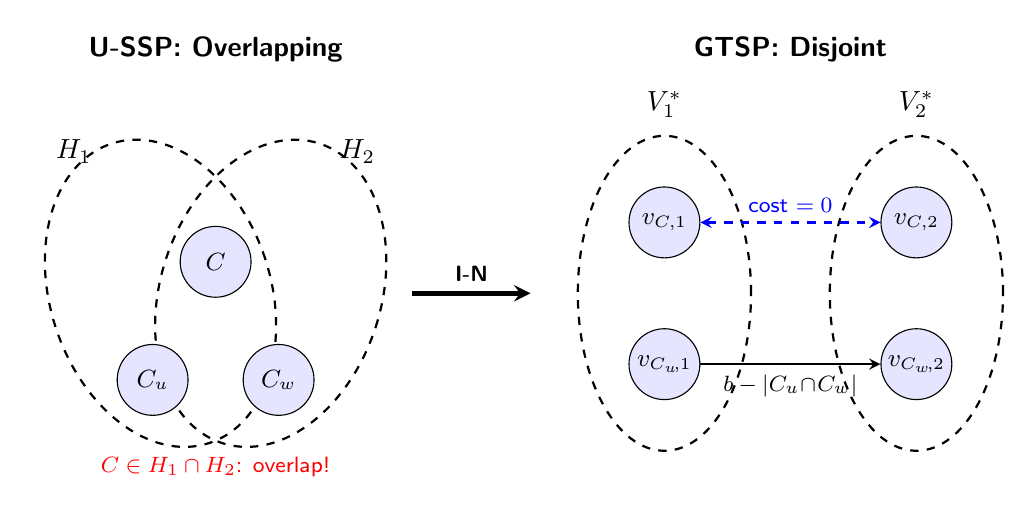
\begin{tikzpicture}[>=stealth, node distance=1.8cm]
  \tikzset{
    clus/.style={draw=black,dashed,thick,ellipse,minimum width=2.6cm,
                 minimum height=4.2cm},
    nod/.style={circle,draw=black,fill=blue!10,minimum size=0.9cm,
                font=\sffamily\small,inner sep=1pt},
    zarr/.style={<->,thick,blue,dashed},
    arr/.style={->,thick,black}
  }
  % Left: SSP overlapping clusters
  \node[font=\sffamily\bfseries] at (-3.5,3.1) {U-SSP: Overlapping};
  \draw[clus,rotate around={18:(-4.2,0)}] (-4.2,0) ellipse (1.4cm and 2.0cm);
  \draw[clus,rotate around={-18:(-2.8,0)}] (-2.8,0) ellipse (1.4cm and 2.0cm);
  \node[font=\sffamily] at (-5.3,1.8) {$H_1$};
  \node[font=\sffamily] at (-1.7,1.8) {$H_2$};
  \node[nod] (c)  at (-3.5, 0.4) {$C$};
  \node[nod] (cu) at (-4.3,-1.1) {$C_u$};
  \node[nod] (cw) at (-2.7,-1.1) {$C_w$};
  \node[font=\sffamily\footnotesize,color=red] at (-3.5,-2.2)
    {$C \in H_1 \cap H_2$: overlap!};

  % Arrow
  \draw[->,ultra thick] (-1.0,0) -- (0.5,0)
    node[midway,above,font=\sffamily\footnotesize\bfseries] {I-N};

  % Right: GTSP disjoint clusters
  \node[font=\sffamily\bfseries] at (3.8,3.1) {GTSP: Disjoint};
  \draw[clus] (2.2,0) ellipse (1.1cm and 2.0cm);
  \draw[clus] (5.4,0) ellipse (1.1cm and 2.0cm);
  \node[font=\sffamily] at (2.2,2.4) {$V_1^*$};
  \node[font=\sffamily] at (5.4,2.4) {$V_2^*$};
  \node[nod] (vc1) at (2.2, 0.9)  {$v_{C,1}$};
  \node[nod] (vu1) at (2.2,-0.9) {$v_{C_u\!,1}$};
  \node[nod] (vc2) at (5.4, 0.9)  {$v_{C,2}$};
  \node[nod] (vw2) at (5.4,-0.9) {$v_{C_w\!,2}$};
  \draw[zarr] (vc1) -- (vc2) node[midway,above,font=\sffamily\footnotesize]{cost $= 0$};
  \draw[arr]  (vu1) -- (vw2)
    node[midway,below,font=\sffamily\footnotesize]{$b-|C_u\!\cap\! C_w|$};
\end{tikzpicture}
\caption{The I-N transformation. Configuration $C$ can process both Job 1
and Job 2 (it is in the intersection $H_1 \cap H_2$). The transformation
creates two distinct replicas $v_{C,1} \in V_1^*$ and $v_{C,2} \in V_2^*$,
linked by a zero-cost arc. Disjointness is achieved without altering any
non-zero transition costs.}
\label{fig:in_transform}
\end{figure}

\subsection{Optimality Preservation}

\begin{thmbox}
\begin{theorem}[SSP–GTSP Bijection \cite{Colares2026Exact}]
\label{thm:bijection}
A minimum-cost Hamiltonian cycle in $\mathcal{I}_{\text{GTSP}}$ corresponds to
an optimal sequence of configurations for $\mathcal{I}_{\text{SSP}}$, with
identical switching cost.
\end{theorem}
\end{thmbox}

\begin{proofbox}
\begin{proof}
Any Hamiltonian cycle in $\mathcal{I}_{\text{GTSP}}$ selects exactly one replica
$v_{C,j}$ from each cluster $V_j^*$, which maps to selecting one configuration
$C \in H_j$ per job — a valid SSP sequence.

Conversely, in any SSP solution, if the magazine stays at configuration $C$ across
a contiguous block of jobs $j_1, j_2, \ldots, j_\ell$, the KTNS policy incurs zero
switches. In the GTSP graph, the replicas $v_{C,j_1}, v_{C,j_2}, \ldots, v_{C,j_\ell}$
are connected by zero-cost arcs, so the GTSP cycle traverses them at zero cost —
exactly mirroring the zero-switch block.

For any transition between distinct configurations $C_u$ and $C_w$, the arc cost
$d^*(v_{C_u,i}, v_{C_w,j}) = b - |C_u \cap C_w|$ equals the number of tool
insertions. Thus the GTSP cycle cost equals the total SSP switching cost, and
minimising the former minimises the latter. \qed
\end{proof}
\end{proofbox}

% ─────────────────────────────────────────────────────────────────────────────
\section{The Disjointness Condition}
\label{sec:disjointness}
% ─────────────────────────────────────────────────────────────────────────────

The I-N transformation inflates the graph size by replicating configurations.
In many instances, however, no replication is needed because the clusters are
already disjoint — the SSP is \emph{natively} a GTSP.

\begin{thmbox}
\begin{theorem}[Disjointness Condition \cite{Colares2026Exact}]
\label{thm:disjoint}
For two distinct jobs $i, k \in J$:
\[
  |T_i \cup T_k| > b \;\implies\; H_i \cap H_k = \emptyset.
\]
\end{theorem}
\end{thmbox}

\begin{proofbox}
\begin{proof}
Suppose for contradiction that $H_i \cap H_k \ne \emptyset$. Then there exists
$C \in \mathcal{C}$ with $T_i \subseteq C$ and $T_k \subseteq C$, so
$(T_i \cup T_k) \subseteq C$. But $|C| = b$, giving
$|T_i \cup T_k| \le |C| = b$, contradicting $|T_i \cup T_k| > b$. \qed
\end{proof}
\end{proofbox}

\begin{corollary}[SSP as a native GTSP]
If $|T_i \cup T_k| > b$ for \emph{every} pair of distinct jobs $i,k \in J$,
then $H_i \cap H_k = \emptyset$ for all $i \ne k$, and the U-SSP maps directly
to a GTSP with disjoint clusters — no I-N replication is needed.
\end{corollary}

\noindent\textbf{Implication.} The standard GTSP is a \emph{special case} of the
SSP (the disjoint-cluster case), not an independent problem. Whenever instances
are ``dense'' (large $|T_j|$ relative to $b$), solvers can be applied without
the overhead of the I-N transformation.

% ─────────────────────────────────────────────────────────────────────────────
\section{The Metric Barrier: Limits of the Reverse Reduction}
\label{sec:metric_barrier}
% ─────────────────────────────────────────────────────────────────────────────

The forward reduction (SSP $\to$ GTSP) is polynomial. A natural question is whether
an arbitrary GTSP can always be reduced back to an SSP. The answer is no, due to
the rigid geometric structure of the SSP metric.

\begin{thmbox}
\begin{theorem}[Metric Barrier \cite{Colares2026Exact}]
\label{thm:barrier}
A GTSP instance with arc weight function $w$ can be polynomially reduced to
a U-SSP only if $w$ satisfies all four properties simultaneously:
\begin{enumerate}[label=(\roman*)]
\item \textbf{Symmetry:} $w(u,v) = w(v,u)$ for all $u,v$.
\item \textbf{Non-negative integer values:} $w(u,v) \in \mathbb{Z}_{\ge 0}$.
\item \textbf{Capacity bound:} $w(u,v) \le b$ for some integer $b$.
\item \textbf{Triangle inequality:} $w(u,v) \le w(u,x) + w(x,v)$ for all $x$.
\end{enumerate}
\end{theorem}
\end{thmbox}

\begin{proofbox}
\begin{proof}
Any SSP transition metric $d(C_u,C_v) = b - |C_u \cap C_v|$ inherits
these four properties:
(i)~symmetry from commutativity of $\cap$;
(ii)~integrality and non-negativity from set cardinalities;
(iii)~$d \le b$ since $|C_u \cap C_v| \ge 0$;
(iv)~the triangle inequality proved in Theorem~\ref{sec:metric} of
\texttt{02\_noncompact\_formulation.tex}.

A GTSP instance violating any one property — e.g., an asymmetric weight
$w(u,v) \ne w(v,u)$, a fractional weight, a weight exceeding $b$, or a
triangle inequality violation — cannot be expressed as $b - |C_u \cap C_v|$
for any integer sets $C_u, C_v$ of size $b$. Since $|C_u \cap C_v|$ is an
integer satisfying $0 \le |C_u \cap C_v| \le b$, no mapping from such a GTSP
to a valid SSP exists. \qed
\end{proof}
\end{proofbox}

\begin{remark}
This barrier is not merely theoretical. Real GTSP instances from routing
applications often have asymmetric costs (direction-dependent travel times),
ruling out direct SSP equivalence. Conversely, SSP instances arising from FMS
scheduling always satisfy all four properties by construction.
\end{remark}

% ─────────────────────────────────────────────────────────────────────────────
\section{Dummy Tool Padding and Metric Symmetry}
\label{sec:dummy_padding}
% ─────────────────────────────────────────────────────────────────────────────

For the restricted GTSP-to-SSP mapping to hold, all configurations must be
maximal (size exactly $b$). Under-capacity states break the symmetry $d(C_u,C_v)=d(C_v,C_u)$ when $|C_u| \ne |C_v|$. Lemma~1 of
\texttt{01\_foundations.tex} ensures this is not an issue: any under-capacity
state can be padded to size $b$ with ``dummy'' tools without increasing cost.
Padding with tools from the \emph{next} group's mandatory set (lookahead padding)
additionally reduces future transition costs, as formalised in
\texttt{05\_jgp\_ssp\_gap\_analysis.tex}.

% ─────────────────────────────────────────────────────────────────────────────
\section{Summary of the SSP–GTSP Relationship}
\label{sec:summary}
% ─────────────────────────────────────────────────────────────────────────────

\begin{center}
\begin{tabular}{lll}
\toprule
Direction & When & Method \\
\midrule
SSP $\to$ GTSP (overlapping) & Always & I-N transformation + zero-cost arcs \\
SSP $\to$ GTSP (disjoint)    & $|T_i \cup T_k|>b$ for all $i \ne k$ & Direct (no replication) \\
GTSP $\to$ SSP & Only if metric satisfies (i)–(iv) & Reverse mapping \\
\bottomrule
\end{tabular}
\end{center}

\noindent The I-N transformation is polynomial in $|\mathcal{C}|=\binom{m}{b}$,
which is exponential in $m$ and $b$. In practice, the column generation approach
of \texttt{02\_noncompact\_formulation.tex} implicitly exploits the GTSP structure
without ever building the full transformed graph.

% ─────────────────────────────────────────────────────────────────────────────
\bibliographystyle{abbrvnat}
\bibliography{references}
% ─────────────────────────────────────────────────────────────────────────────
\end{document}
